\section{LP-Rounding for \robcc}
In this section, we design efficient bi-criteria approximation algorithms for \robcc (\Cref{prob:2}), thereby proving~\Cref{thm:complete1,thm:complete2}. We begin by recalling the problem setup: we are given an instance ${\cal I}$ of \robcc consisting of a graph $(V, E_{+}, E_{-})$ on $n$ points, where $E_{+}$ denotes the set of pairs of vertices which are similar to each other, and $E_{-}$ denotes the dissimilar pairs (since the problem is over complete graphs, we additionally have that $E_{+} \cup E_{-} = \binom{[n]}{2}$). The goal is to identify a set of vertices $D$ such that $|D| = m$, and a clustering $\mathcal{C}$ over $V\setminus D$ such that the total cost (number of $E_{+}$ edges going between clusters and $E_{-}$ edges staying within a cluster) of $\mathcal{C}$ is minimized.

The main result of this section is an LP-based approximation algorithm, whose starting point is the following natural LP relaxation of the problem. In the LP relaxation below, there is a variable $z_{u,v}$ for each pair $(u,v)$ of vertices, which is the relaxation of the indicator variable for whether the corresponding edge is an edge the optimal solution will misclassify, i.e., it will be $1$ if the endpoints $u$ and $v$ are in different clusters and $(u,v) \in E_{+}$ \emph{or} if the endpoints $u$ and $v$ are in the same cluster and $(u,v) \in E_{-}$, and $0$ otherwise. The variable $y_u$ for each vertex $u$ denotes whether the optimal solution declares $u$ to be an outlier or not. Finally, there is a variable $x_{u,v}$ which denotes the cut-metric induced by the optimal clustering, i.e., $x_{u,v} = 1$ if and only if $u$ and $v$ are in different clusters of the clustering. 

\begin{alignat}{3} \label{LP:CC5}
		\text{minimize} &\sum_{(u,v) \in E} z_{u,v}, && \quad s.t., \tag{LP5}\\
		x_{u,v} &\le x_{u,w} + x_{v,w}, &&\qquad \forall u,v,w \in [n], \label{LP:CC5:1}\\
		y_u + y_v + z_{u,v} &\ge x_{u,v},&&\qquad \forall (u,v) \in E^+, \label{LP:CC5:1}\\
		y_u + y_v + z_{u,v} &\ge 1 - x_{u,v}, &&\qquad \forall (u,v) \in E^-, \label{LP:CC5:1}\\
		\sum_{u} y_u &\le m, \label{LP:CC5:1} \\
		x_{u,v} &\in [ 0,1 ], &&\qquad \forall u,v \in [n], \nonumber\\
		z_{u,v} &\in [ 0,1 ], &&\qquad \forall u,v \in [n],\nonumber\\
		y_u &\in [ 0,1 ], &&\qquad \forall u \in [n]. \nonumber
\end{alignat}

\begin{lemma} \label{lem:relaxation1}
The LP \Cref{LP:CC5} is a valid LP relaxation for the \robcc problem. In other words, the objective value of an optimal LP solution is at most $\opt({\cal I})$, where $\opt({\cal I})$ is the objective value of an optimal \robcc solution to instance ${\cal I}$.
\end{lemma}

\begin{proof}
Proof is here.
\end{proof}


Our algorithm will in fact be based on a different LP relaxation for the problem, which is a natural extension of a very elegant LP relaxation for the original correlation clustering problem. We start with the following definition, which will be useful throughout the algorithm and analysis.
\begin{definition}
A triplet $(u,v,w)$ of points is said to be a \emph{bad triangle} if exactly two of the three edges among $(u,v), (v,w), (u,w)$ belong to $E_{+}$ and one to $E_{-}$. In words, there is exactly one negative edge in the triangle formed by $u, v$ and $w$.
 \end{definition}

Intuitively, a bad triangle captures the smallest unit of inconsistency in the similarity information among the given points. Indeed, irrespective of how the vertices of a bad triangle are clustered, note that the edges of this triangle incur a cost of at least $1$ unit in the objective function. This intuition is the crux behind the following LP relaxation of Charikar et al~\cite{XXX}. In what follows, let ${\cal B}$ denote the set of all bad triangles in the instance ${\cal I}$.

\begin{alignat}{3} \label{LP:robcc-triangles}
    \text{minimize} \sum_{(u,v) \in \binom{V}{2}} z_{u,v},& &&s.t. \label{LP3} \tag{LP_{\robcc}}\\
    y_u + y_v + y_w + z_{u,v} + z_{v,w} + z_{u,w} \ge 1,& &&\forall T \equiv (u,v,w) \in {\cal B} , \nonumber\\
    \sum_{u} y_u \le m, & \nonumber\\
	z_{u,v} \in [ 0,1 ]&\qquad && \forall (u,v) \in \binom{V}{2}, \label{eq:011} \\
	y_u \in [0,1]&, && \forall u \in V. \label{eq:002}
\end{alignat}

\begin{lemma} \label{lem:relaxation-triangles}
The LP \Cref{LP:robcc-triangles} is a valid LP relaxation for the \robcc problem, and the objective value of an optimal LP solution is at most $\opt({\cal I})$, where $\opt({\cal I})$ is the objective value of an optimal \robcc solution to instance ${\cal I}$.
\end{lemma}

\begin{proof}
Proof is here.
\end{proof}


% 		\min \qquad \sum_{i \in F, j \in C}x_{i, j} d^q(i, j) \tag{$\text{LP}_{\text{strong}}$} \qquad  \label{LP:strong}
% 	\text{s.t.} \\
% 		y_i &= 1 & & \forall i \in S_0 &\label{LPs:S0}\\
% 		 x_{i,j} &= 0 & &\forall i, j \, \text { s.t } \, d(i,j) >  R_j & \label{LPs:R} \\
% 	    \sum_{j} d^q(i,j) x_{i,j} & \leq \rho \tilde U y_i & & \forall i \notin S_0 & \label{LPs:star} \\[-6pt]
% 	    x_{i,j} &= 0 & &\forall i \notin S_0, j \, \text { s.t } \, d^q(i,j) >  \rho \tilde U &\label{LPs:R-d}

\subsection{Rounding Algorithm}
Let $\Opt_{\Cref{LP3}} = \{ z^*_{u,v}, y^*_u \}$ denote the fractional optimal solution of this linear program.

\begin{algorithm}
\caption{${\sf RCC}(V,\sigma,m)$}
\label{alg:RCC}
\begin{algorithmic}[1]
\State \textbf{Input:} Dataset $V$; correlation clustering instance $\sigma : \binom{V}{2} \to \{ +,- \}$.
\State \textbf{Initialization:} $V_{g} = V$ \Comment{Set of unremoved vertices}
\State Let the optimal solution of \ref{LP3} be denoted as $\{ Y_u^* : u \in V\} \cup \{ x_{uv}^* : (u,v) \in \binom{V}{2} \}$
\For{$v \in V : Y_v^* \ge \frac14$}
\State $V_{g} \gets V_{g} \setminus \{ v \}$
\Comment{Delete vertices having $Y_u^* \ge 1/4$}
\EndFor
\State Let $\sigma_g$ be the restriction of $\sigma$ to vertices in $V_g$.
\State \textbf{Return:} Clustering ${\sf CharikarCC} (V_g,\sigma_g)$.
\end{algorithmic}
%\end{center}
\end{algorithm}

\begin{algorithm}
\caption{${\sf CharikarCC}(V,\sigma)$}
\label{alg:CharikarCC}
\begin{algorithmic}
\State \textbf{Input:} Dataset $V$; correlation clustering instance $\sigma : \binom{V}{2} \to \{ +,- \}$.
\State \textbf{Initialization:} $V_{nc} = V$. \Comment{Set of unclustered points among $V$}
\While{$V_{nc} \ne \phi$}
\State Sample $v \sim \mathrm{Unif} (V_{nc})$.
\State Define $C(v) = \{ u \in V_{nc} : \sign (u,v) = +\} \cup \{ v \}$ \Comment{Vertices similar to $v$ including $v$}
\State $V_{nc} \gets V_{nc} \setminus C(v)$.
\EndWhile
\end{algorithmic}
%\end{center}
\end{algorithm}

\begin{theorem}
${\sf CharikarCC}(V,\sigma)$ is a $3$ approximation for Correlation Clustering.
\end{theorem}
\begin{proof} Let $t$ denote the triple $(u,v,w)$ where $\Delta uvw$ forms a bad triangle with two positive edges and one negative edge. Let $A_t^{(i)}$ denote the event that in iteration $i$, one of $u,v,w$ is chosen as a pivot and that $u,v,w$ belong to $V'$ in this recursive call of the algorithm. The total cost of the algorithm is then $\sum_i \sum_t \mathbbm{1} (A_t^{(i)})$. Using $A_t$ to represent the event that one of $u,v,w$ is chosen as a pivot in some iteration and that $u,v,w$ belong to $V'$ in the same recursive call of the algorithm, its cost can be written as $\sum_t \mathbbm{1} (A_t)$. Therefore, the expected cost of the algorithm is $\sum_t p_t$ where $p_t$ is the probability of the event $A_t$ occurring.\\

\noindent Observe that any algorithm will have to pay a unit cost for each triangle among any set of edge disjoint triangles from $B$. Therefore, we construct an optimization problem that finds the maximum number of edge disjoint triangles from $B$ and conclude that the cost of $OPT$ is at least this much. Let $B$ denote the set of tuples $(u,v,w)$ corresponding to bad triangles $\Delta uvw$. We therefore consider the dual to a relaxed LP,

\begin{alignat}{3} \label{LP:CC-relax-dual}
		\text{maximize} \qquad \sum_{t \in B} z_t &, && \qquad s.t., \nonumber\\
		\sum_{t \in B : u,v \in t} z_t \le 1& , &&\qquad \forall e = (u,v) \in E , \nonumber\\
		z_{t} \in [ 0,1 ]&, &&\qquad \forall t \in B,.\tag{LP1}
\end{alignat}

We now show that the set of probabilities $\{ p_t / 3,\ t \in B \}$ forms a valid solution to this LP. This proves that the algorithm is $3$ approximate since any solution to \ref{LP:CC-relax-dual} is a lower bound to $OPT$. Consider any edge $e = (u,v)$ and the bad triangles $B_{uv} = \{ t_w : (u,v,w) \in B \}$ it is part of. For any of these bad triangles, if the third vertex $w$ is picked as a cluster center then $(u,v)$ will become misclassified. The probability that $w$ is picked conditioned on $A_{t_w}$ is $1/3$. Therefore, we have:
\begin{equation} \label{eq:0000}
    P ( (u,v) \text{ is misclassified}) = \sum_{t \in B_{uv}} \frac{1}{3} p_t.
\end{equation}
Therefore, for every edge $e = (u,v)$, $\sum_{t \in B_{uv}} \frac{1}{3} p_t \le 1$ and this forms a feasible fractional solution to \ref{LP:CC-relax-dual}.
\end{proof}

% \begin{figure}[H]
% \centering
% 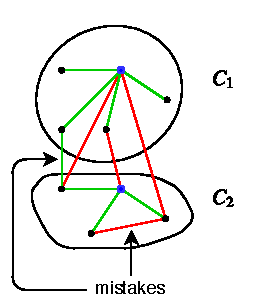
\includegraphics{./img/3apx.pdf}
% \caption{An instance of Algorithm \ref{alg:CC:3apx}}
% \label{fig:5}
% \end{figure}



%%%%%%%%%%%%%%%%%%%%%%%%%%%%%%%%%%%%%%%%%%%%%%%%%%

\subsection{LP-rounding based approximation for $m$-Robust Correlation Clustering}

We use the notation \textit{$(\alpha, \beta)$ bi-criterion approximation} to denote an algorithm for $m$-Robust Correlation Clustering which removes at most $\alpha m$ points, generating a solution within a factor of $\beta$ of the optimal cost. In the following, we describe a simple LP-rounding based $(4,12)$ bi-criteria approximation for $m$-Robust Correlation Clustering.


\begin{theorem}
Algorithm ${\sf RCC} (V,\sigma,m)$ is a $(4,12)$ bi-criteria approximation for $m$-Robust Correlation Clustering.
\end{theorem}
\begin{proof}
In order to show that ${\sf RCC} (V,\sigma,m)$ is a $(4,12)$ bi-criteria approximation for $m$-Robust Correlation Clustering, we show that (a) at most $4m$ vertices are deleted, and (b) the clustering has a cost within a factor of $12$ of the optimal.

\begin{enumerate}
    \item[(a)] According to ${\sf RCC}(V,\sigma,m)$, vertices having $Y_u^* \ge 1/4$ in the optimal LP solution are deleted. Let the set of vertices deleted by ${\sf RCC} (V,\sigma,m)$ be denoted $V_r$. Then,
    \begin{align*}
        |V_r| &= \sum_{u \in V} \mathbbm{1} (Y_u^* \ge 1/4)\\
        &\le \sum_{u \in V} 4 Y_u^*\\
        &\le 4m
    \end{align*}
Therefore, the budget of number of vertices removed is not exceeded by more than a factor of $4$.\\

In order to show that the cost is within a factor of $12$ of the optimal, recall the definition of \ref{LP3} which is an LP relaxation for the $m$-Robust Correlation Clustering LP. 
On the other hand, for any vertex that is removed, the corresponding bad triangles do not incur any cost for the algorithm. In case, none of the vertices of the triangle are removed, the constraints of \ref{LP3} are now represented as:
\begin{alignat}{3} \label{LP:CC-relax-reduced:2}
		\text{minimize} \qquad \sum_{(u,v) \in \binom{V}{2} : Y_u^*, Y_v^* \le 1/4} z_{uv}&, \qquad &&s.t., \nonumber\\
		\quad z_{uv} + z_{vw} + z_{uw} \ge 1/4 &, \qquad &&\forall t = (u,v,w) \in B : Y_u^* \ \&\ Y_v^* \ \&\ Y_w^* \le 1/4, \nonumber\\
		z_{uv} \in [ 0,1 ]&, \qquad &&\forall (u,v) \in \binom{V}{2}. \tag{LP4}
\end{alignat}
Let $B'$ represent the set of triples $(u,v,w)$ in $B$ such that $Y_u^* \ \&\ Y_v^* \ \&\ Y_w^* \le 1/4$.
The dual of this LP is:
\begin{alignat}{3} \label{LP:CC-relax-reduced-dual:2}
		\text{maximize}\qquad \frac{1}{4} \sum_{t \in B'} r_t &, && \qquad s.t., \nonumber\\
		\sum_{t \in B' : u,v \in t} r_t \le 1 &, &&\qquad \forall e = (u,v) \in E, \nonumber\\
		r_{t} \in [ 0,1 ] &, &&\qquad \forall t \in B'.\tag{LP5}
\end{alignat}
By a similar logic as previously, the solution $\{ \frac{1}{3} p_t, t \in B'\}$ is a valid solution to the dual, having cost equal to $\frac{1}{12} \sum_{t \in B'} p_t$. The algorithm has an expected cost of $\sum_{t \in B'} p_t$. This is because the algorithm only accumulates the cost corresponding to the event $A_t$ if none of the vertices in $t$ are removed in the preliminary vertex removal stage.
    \item[(b)]
\end{enumerate}

\end{proof}


\subsection{A combinatorial approximation for $m$-Robust Clustering on complete graphs}

The linear programming relaxation of \ref{IP:CC5} is obtained by replacing the integer constraints in \eqref{eq:d01}, \eqref{eq:d02}, and \eqref{eq:d03} by $x_{uv} \in [0,1]$, $z_{uv} \in [0,1]$, and $Y_u \in[0,1]$ respectively. Let \setword{LP4}{LP:CC-relax-ip4} denote this relaxed LP, and $\opt^*$ denote the optimal solution to \ref{LP:CC-relax-ip4}. Let us consider the following relaxation to \ref{LP:CC-relax-ip4},

\begin{alignat}{3} \label{LP:CC-relax:3}
		\text{Minimize} \qquad \sum_{(u,v) \in \binom{V}{2}} x_{uv} + \frac{OPT^*}{m} \sum_u Y_u &, \qquad &&s.t., \nonumber\\
		Y_u + Y_v + Y_w + z_{uv} + z_{vw} + z_{uw} \ge 1 &, \qquad &&\forall t = (u,v,w) \in B, \nonumber\\
		z_{uv} \in [ 0,1 ]&, \qquad &&\forall (u,v) \in \binom{V}{2}, \nonumber\\
		Y_u \in [0,1] &,\qquad  &&\forall u \in V. \tag{LP6}
\end{alignat}

\noindent We know that the optimal solution to \ref{LP:CC-relax:3} is within a factor of $2$ of the optimal solution to \ref{LP:CC-relax-ip4}. This is because the optimal solution of \ref{LP:CC-relax-ip4} is a feasible solution to \ref{LP:CC-relax:3} with a cost of $2*\opt^*$. The dual of \ref{LP:CC-relax:3} is:

\begin{alignat}{3} 
		\text{Maximize} \qquad \sum_{t \in B} w_t &, \qquad&&s.t., \label{LP:CC-relax-dual:3} \tag{LP7}\\
		\sum_{t : u,v \in t} w_t \le 1 &, \qquad&&\forall u,v \in \binom{V}{2}, \label{eq:d04}\\
		\sum_{t : u \in t} w_t \le \frac{OPT^*}{m}&, \qquad&&\forall v \in V, \label{eq:d05}\\
		w_t \ge 0&, \qquad &&\forall v \in V. \nonumber
\end{alignat}

% \begin{algorithm} \label{alg:IP:CC7}
% Run Charikar clustering. Delete vertices which are connected to at least $OPT^* / m$ mis-classified edges.
% \end{algorithm}

\begin{algorithm}
\caption{{\sf RCC-Comb}$(V,\sigma,m)$}
\label{RCC-Comb}
\begin{algorithmic}[1]
\State \textbf{Input:} Dataset $V$; correlation clustering instance $\sigma : \binom{V}{2} \to \{ +,- \}$.
%\State \textbf{Initialization:} $V_r = V$ \Comment{Set of unremoved vertices}
\State \textbf{Initialization:} $V_r = \phi$; $\forall v\in V,\ Counter_v=0$; \Comment{$V_r$ is the set of removed vertices}
\Statex \hskip7em Mark all bad triangles $untouched$
\State $\mathcal{C} = {\sf CharikarCC} (V,\sigma)$.
\State Let $A$ be the ordered set of vertices sampled in $\mathcal{C}$
\For{$v \in A$}
\While{$\exists \; untouched$ bad triangle $t=(u,v,w) : u,v,w \not\in V_r$}
\State Mark the bad triangle $t$ as $touched$.
\State $Counter_u \gets Counter_u +1$
\State $Counter_v \gets Counter_v +1$
\State $Counter_w \gets Counter_w +1$
\For{$v'\in \{u,v,w\}$}
\If{$Counter_{v'} \geq 3\opt^* / m$}
\State $V_r \gets V_r \cup \{ v' \}$
%\State $\mathcal{C} \gets \mathcal{C} \setminus v'$ \Comment{Remove vertex $v'$ from the clustering $\mathcal{C}$}
\EndIf
\EndFor
\EndWhile
\EndFor
% \State Let the optimal solution of \ref{LP3} be denoted as $\{ Y_u^* : u \in V\} \cup \{ x_{uv}^* : (u,v) \in \binom{V}{2} \}$
% \For{$v \in V : Y_v^* \ge \frac14$}
% \State $V_{g} \gets V_{g} \setminus \{ v \}$
% \EndFor
% \State Let $\sigma_g$ be the restriction of $\sigma$ to vertices in $V_g$.
% \State \textbf{Return:} Clustering ${\sf CharikarCC} (V_g,\sigma_g)$.
\State \textbf{Return:} Clustering $\mathcal{C}$, $V_r$
\end{algorithmic}
%\end{center}
\end{algorithm}

\begin{theorem} \label{theorem:rcc-comb}
{\sf RCC-Comb}$(V,\sigma,m)$ is a $(6,6)$ bi-criteria approximation for $m$-robust correlation clustering.
\end{theorem}
\begin{proof}
Let $p_t'$ be the probability that a bad triangle is touched in {\sf RCC-Comb}$(V,\sigma,m)$. Also let $w_t = \frac{p_t'}{3}$ in \ref{LP:CC-relax:3}. We show that cost of the algorithm {\sf RCC-Comb}$(V,\sigma,m)$ is $\leq \sum_t p_t'$, which using the duality property is bounded by $2\opt^*$. We also show that $w_t = \frac{p_t'}{3}$ satisfies constraints \eqref{eq:d04} and \eqref{eq:d05}, and provides a bound on the number of vertices deleted in the algorithm {\sf RCC-Comb}$(V,\sigma,m)$. The proof of these statements are presented through Lemma \ref{RCC:l1}, Lemma \ref{RCC:l2}, Lemma \ref{RCC:l3}, and Lemma \ref{RCC:l4}.
\end{proof}

\begin{lemma} \label{RCC:l1}
$w_t = \frac{p_t'}{3}$ satisfies equation \eqref{eq:d04}.
\end{lemma}
\begin{proof}
Proof follows from \eqref{eq:0000}, and the fact that $p_t' \leq p_t$ since we go over the vertices in same order as sampled in {\sf CharikarCC}$(V,\sigma)$. Recall that $A_t$ refers to the event that one of $u,v,w \in t$ is chosen while sampling vertices in {\sf CharikarCC}$(V,\sigma)$. Hence the event $A_t$ should occur for the triangle $t$ to be touched in Algorithm \ref{RCC-Comb}.
\end{proof}

\begin{lemma}\label{RCC:l2}
$w_t$ = $\frac{p_t'}{3}$ satisfies equation \eqref{eq:d05}.
\end{lemma}
\begin{proof}
For a vertex $u$, $Counter_u$ is incremented when any bad triangle that contains $v$ is touched. Therefore,
\begin{equation*}
    \mathbb{E} [Counter_u] = \mathbb{E} \left[ \sum_{t : u \in t} \mathbbm{1} (t \text{ is touched}) \right] = \sum_{t : u \in t} p_t'
\end{equation*}
Since $Counter_u$ for any vertex $u$ does not exceed $\frac{3\opt^*}{m}$, from \eqref{eq:d05} it follows that:
\begin{equation} \label{eq:d06}
    \sum_{t : u \in t} \frac{p_t'}{3} \le \frac{ \opt^*}{m}
\end{equation}
Recall that the dual solution under consideration is $\{ w_t : t \in B\} = \{ p_t'/ 3 : t \in B\}$. Therefore, from \eqref{eq:d06},
\begin{equation*}
\sum_{t : u \in t} w_t \leq \frac{\opt^*}{m}
\end{equation*}
\end{proof}

\begin{lemma}\label{RCC:l3}
The number of deleted vertices in {\sf RCC-Comb}$(V,\sigma,m)$ is $\leq 3m$.
\end{lemma}
\begin{proof}
Let $B$ denote the set of bad triangles. Then,
\begin{align}
    \frac{3\opt^*}{m} \mathbb{E}\left[\# \text{ deleted vertices}\right] &\leq \sum_{v\in V}Counter_v \nonumber
\end{align}
We know that every time a triangle $t=(u,v,w)$ is touched, the counters $Counter_u, Counter_v, Counter_w$ gets incremented by $1$. Hence every touched triangle $t$ contributes an increment in counter of $3$ vertices in the $\sum_{v\in V}Counter_v$.
\begin{align}
    %\overset{(i)}{\leq}
    \frac{3\opt^*}{m} \mathbb{E}\left[\# \text{ deleted vertices}\right] &\leq \sum_{t\in B}3\mathbb{E}[\mathbbm{1}(t\text{ is touched})] \nonumber\\
    & \leq 3\sum_{t\in B}p_{t'} = 9\sum_{t\in B}w_{t'} \nonumber
\end{align}
By LP duality, we have that $\sum_{t\in B}w_{t'} \leq \opt(\ref{LP:CC-relax:3})$, which is itself $\leq 2\opt^*$. Hence,
\begin{align}
    \frac{3\opt^*}{m} \mathbb{E}\left[\# \text{ deleted vertices}\right] &\leq 18\opt^* \nonumber \\
    \implies \mathbb{E}[\# \text{ deleted vertices}] &\leq 6m. \nonumber
\end{align}
\end{proof}

\begin{lemma}\label{RCC:l4}
Let $\alg$ indicate the cost of {\sf RCC-Comb}$(V,\sigma,m))$. Then,
\begin{equation*}
    \alg \le 6\opt^*
\end{equation*}
\end{lemma}
\begin{proof}
Let $T$ represent the set of triangles $t = (u,v,w)$ are touched and such that none of vertices $u,v,$ or $w$ are deleted in {\sf RCC-Comb}$(V,\sigma,m)$. The cost of {\sf RCC-Comb}$(V,\sigma,m)$ is equal to $|T|$. Let $p_t''$ represent the probability that $t \in T$. Then,
\begin{equation}
    \alg = \mathbb{E}[|T|] = \sum_t \mathbbm{1} (t \in T) = \sum_{t} p_t'' \label{eq:d07}
\end{equation}
But in order for a triangle $t$ belong in $T$, it needs to be touched. Therefore, $p_t'' \leq p_t'$, and from \eqref{eq:d07}, it follows that
\begin{equation} \label{eq:d08}
\alg \leq \sum_t p_t'.
\end{equation}
Recall that the dual solution we consider in \ref{LP:CC-relax-dual:3} is $w_t = p_t' / 3$. Then by the duality of \ref{LP:CC-relax:3} and, we get
\begin{align}
    \sum_t p_t' = 3 \sum_t w_t &\leq 3 \opt (\ref{LP:CC-relax:3})\nonumber\\
    &\le 6\opt^*. \label{eq:d09}
\end{align}
The proof concludes by combining \eqref{eq:d08} and \eqref{eq:d09}. 
\end{proof}


% \noindent For brevity, let the function $\mathrm{Mis} (v)$ count the number of mis-classified edges associated with vertex $v$ in a clustering. After using Charikar's clustering, the expected number of mis-classified edges vertex $u$ is connected to is equal to, 
% \begin{align} 
%     \mathbb{E} [\mathrm{Mis} (u)] &= \sum_{v \ne u} P( (u,v) \text{ is misclassified})\\
%     &= \sum_{v \ne u} \sum_{t : u,v \in t} p_t \qquad [\text{from Equation } \eqref{eq:0000}] \nonumber\\
%     &= \sum_{t : u \in t} p_t. \label{eq:00004}
% \end{align}
% Using Markov's inequality, the probability that the vertex is deleted in the next round is:
% \begin{align*}
%     P (u \text{ is deleted}) &= P \left( \mathrm{Mis} (u) \ge \frac{OPT^*}{m} \right) \\
%     &\le \frac{m}{OPT^*} \cdot \mathbb{E} [\mathrm{Mis} (u)]
% \end{align*}
% Therefore, the expected number of deleted vertices is:
% \begin{align}
%     \mathbb{E} [\# \text{ deleted vertices}] &\le \sum_u \frac{m}{OPT^*} \mathbb{E} [\mathrm{Mis} (u)] \nonumber\\
%     &= \frac{m}{OPT^*} \sum_u \underbrace{\sum_{t : u \in t} p_t}_{\text{defined as } Z_u} \qquad [\text{ from Equation } \eqref{eq:00004} ] \nonumber\\
%     &\le 3m \frac{\sum_t p_t}{OPT^*} \label{eq:0001}
% \end{align}
% The last inequality uses the fact that any $p_t$ may appear in at most $3$ different $Z_u$'s. Therefore, $\sum_u Z_u \le 3\sum_t p_t $. The RHS of Equation \eqref{eq:0001} is the ratio of Charikar's clustering to the optimal fractional solution of \ref{LP:CC-relax:2} which are known to be within a factor of $3$. Therefore,
% \begin{equation*}
%     \mathbb{E} [\# \text{ deleted vertices}] \le 9m
% \end{equation*}
% On the other hand, the expected cost of the algorithm is equal to:
% \begin{equation} \label{eq:0003}
%     ALG = \mathbb{E} \left[ \sum_{t : t \cap R = \phi} p_t \right],
% \end{equation}
% where $R$ is the random set of vertices that are connected to at least $OPT^* / m$ mis-classified edges. Every bad triangle $t$ that is counted in Equation \eqref{eq:0003} does not have more than $OPT^*/m$ mis-classified edges associated with each of its vertices. The cost in Equation \eqref{eq:0003} can be rewritten as,
% \begin{equation}
%     \mathbb{E} [ALG] = \sum_{t \in B} p'_t,
% \end{equation}
% where $p_t'$ is defined as $P \left( A_t \ \& \ \mathrm{Mis} (u) \le \frac{OPT^*}{m} \ \& \ \mathrm{Mis}(v) \le \frac{OPT^*}{m} \ \&\ \mathrm{Mis} (w) \le \frac{OPT^*}{m} \right)$, the probability that the cost of the bad triangle is counted after vertex deletion.
% Consider the solution $ \mathbf{S}$ equal to $\{ p_t' / 3 : t \in B \}$. We show that this is a feasible solution to the relaxed dual \ref{LP:CC-relax-dual:3}. The edge constraints are satisfied by the same previous arguments since $p_t' \le p_t$. Consider any vertex constraint of \ref{LP:CC-relax-dual:3},
% \begin{align*}
%     \sum_{t : u \in t} z_t = \frac{1}{3} \sum_{t : u \in t} p_t'.
% \end{align*}
% This is equal to $1/3$ times the average number of mis-classified edges connected to $u$ after the vertex deletion stage (observe Equation \eqref{eq:00004} to understand) which itself cannot exceed $OPT^* / m$ (by the vertex deletion criterion).
% Therefore, the cost of $\mathbf{S}$ lower bounds the optimal fractional solution of \ref{LP:CC-relax:3}. It is known that this does not exceed twice of $OPT^*$ which we benchmark our algorithm's cost against. Therefore, we have from \eqref{eq:0003} that,
% \begin{align*}
%     \frac{\mathbb{E} [ALG]}{OPT^*} \le 2 \frac{\mathbb{E} [ALG]}{OPT_{\ref{LP:CC-relax:3}}} &\le 2 \frac{\mathbb{E} [ALG]}{OPT_{\ref{LP:CC-relax-dual:3}}} \\
%     &\le 2\frac{\mathbb{E} [ALG]}{\cost (\mathbf{S})} \\
%     &= 6
% \end{align*}